\subsection{Regular Expressions in Streaming}
\begin{frame}
  \centering
  {\Large Streaming Regular Expression Membership and Pattern Matching}

  \bigskip
  {\large SODA'22}\\
  \bigskip
  
\includegraphics{pictures/mindmap/regexp.png}

  \bigskip
  Bartłomiej Dudek, Paweł Gawrychowski, Tatiana Starikovskaya
\end{frame}

\begin{frame}{A powerful matching model: regular expressions}
    \begin{columns}
        \column{.6\textwidth}
        \begin{mydefblock}{Regular expressions (regexp)}
            either a character from $\Sigma$ or recursively defined from other regular expressions $R_1$ and $R_2$:
            %\pause
            \begin{enumerate}
                \item $R_1 \cdot R_2$ (concatenation),
                %\pause
                \item $R_1 | R_2$ (union),
                %\pause
                \item $R_1^\ast$ (Kleene star).
            \end{enumerate}
        \end{mydefblock}
        \pause
        \column{.4\textwidth}
        \begin{center}
            %\only<1|handout:0>{\textbf{Ex:} For $\Sigma=\{a,b\}$,\\ 
            % $R_1=a$ only matches $a$,\\
            % and $R_2=b$ only matches $b$.}
            %\only<2|handout:0>{$R_1 \cdot R_2$ matches anything matching $R_1$ followed by anything matching $R_2$.\\
            %\textbf{Ex:} with $R_1=a$ and $R_2=b$, $R_1 \cdot R_2$ matches $ab$.}
            %\only<3|handout:0>{$R_1 | R_2$ matches anything matching $R_1$ or  $R_2$.\\
            %\textbf{Ex:} with $R_1=a \cdot b = ab$ and $R_2=b$, $R_1 | R_2$ matches $ab$ and $b$.}
            %\only<4|handout:0>{$R_1^\ast$ matches any number of repetition of any string matching $R_1$.\\
            %\textbf{Ex:} with $R_1=(b|ab)$ matches $\varepsilon$, $ab$, $b$, $bbabb$...}
            %\only<5->{
                \textbf{Ex:} $b(b|ab)^\ast ab$\\
                \smallskip
                \cmark ~ $bbbbbabab$ \\
                \cmark ~ $bbbabbbbab$\\
                \xmark ~ $bbbaabbbab$\\
                \xmark ~ $baba$\\ 
                \xmark ~ $abab$\\
            %    }
        \end{center}
    \end{columns}    
    %\pause
    %\pause

    \bigskip
    Used in databases, \pause data mining, \pause secret detection, \pause computer networks, \pause protein search\pause ...\\
    \pause
    \bigskip
    {
        \beamermathcolor{myblue}
        Given a regular expression $R$ and a string $T$, \bblue{membership} is : check if $R$ matches $T$.\\
        %\bblue{Pattern matching:} check if $R$ matches \textbf{some substring} of $T$. \pause \\
        %\textcolor{myblue}{Reduces to membership!}
    }
    
    
    \pause
    \medskip
    We define the length of $R$ to be the number of $\cdot$, $|$, and $\ast$ that it contains.
\end{frame}

\begin{frame}{A frugal model of computation: Streaming}
\begin{columns}
    \column{.4\textwidth}
    The algorithm first receives and preprocesses the expression.\\ Next, it keeps reading characters from a very very long string and:
    \column{.5\textwidth}
    \begin{center}
        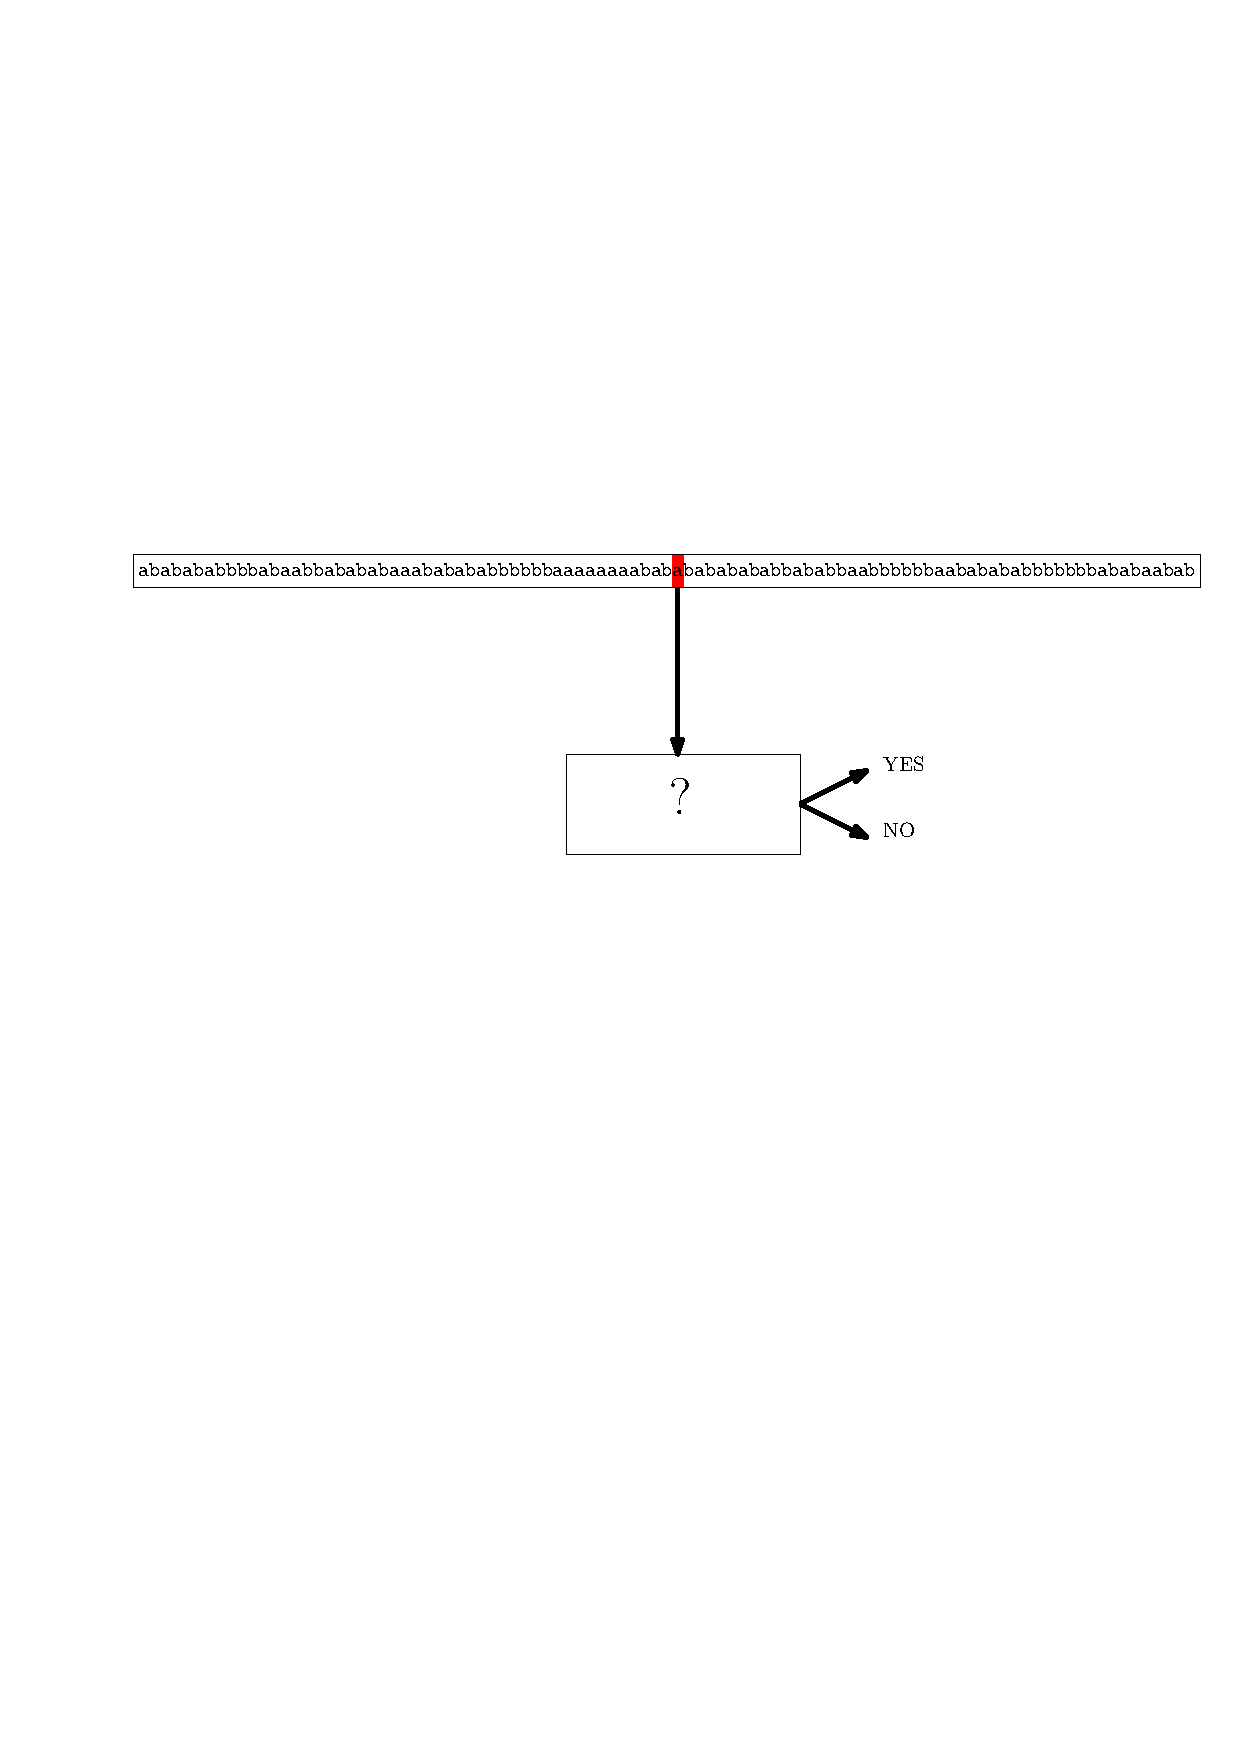
\includegraphics[width=\textwidth]{pictures/stream3}
    \end{center}
\end{columns}

\smallskip
\pause
\begin{enumerate}
\item \textbf{No delay:} After having seen the $i$-th character, immediately report whether the string so far matches the regular expression.
\pause
\item \textbf{No going back:} Not possible to read any of the earlier characters.
\pause
\item \textbf{Every space counts:} No access to the original expression (unless stored explicitly).
\end{enumerate}
\pause
\begin{center}
    \small
    A crucial  tool is the variant of Karp--Rabin fingerprints of \ntheme{[Porat and Porat, FOCS'09]}.
\end{center}\pause
\begin{mylemblock}{Classic pattern matching in streaming [Breslauer and Galil, TALG'14]}
    For a pattern of length $m$, it takes $\Oh(\log m)$ space and $\Oh(1)$ time per position.
\end{mylemblock}

\end{frame}

\begin{frame}{State of the art on regular expression membership}
    \begin{columns}
        \column{.4\textwidth}
        For a regexp of length $m$,\\
        \ntheme{Classic:} Recursively build the \btheme{Thompson automata}, then check if $T$ is accepted.\\
        $\Oh(m)$ space and time/character.
        \column{.5\textwidth}
        \centering
        \begin{picture}(200,65)
            \put(0,0){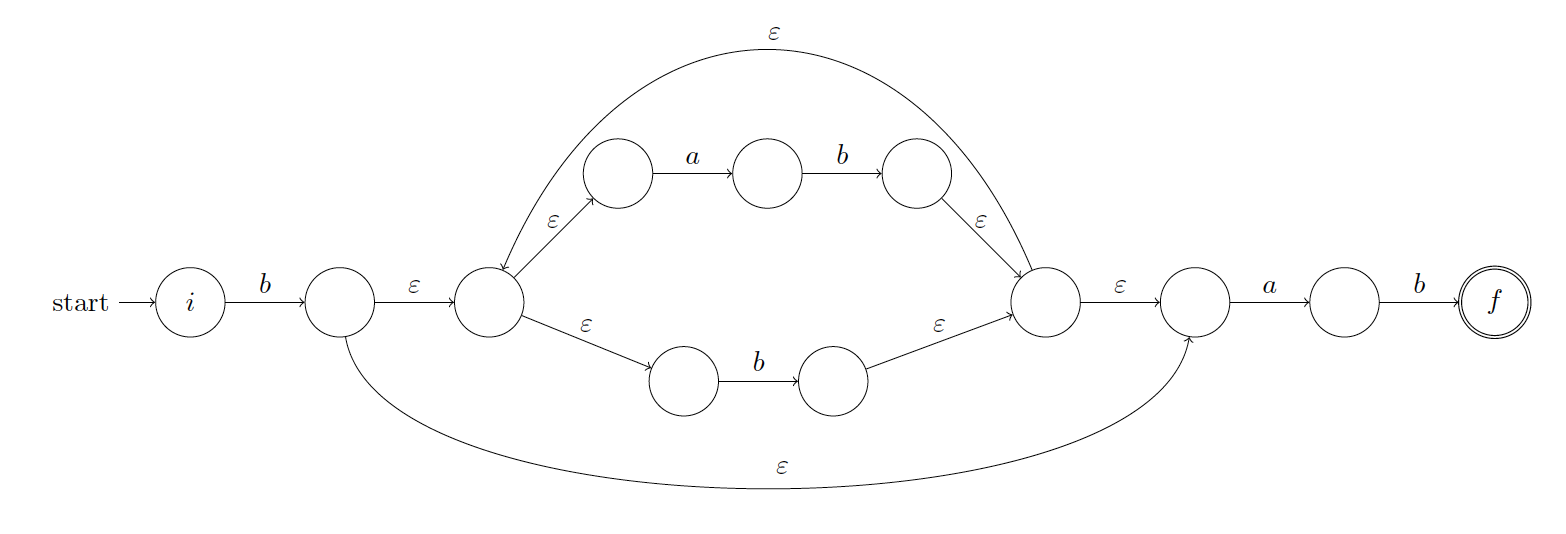
\includegraphics[width=\textwidth]{pictures/thomson1.png}}
            \put(150,50){\small $b(b|ab)^\ast ab$}
        \end{picture}
    \end{columns}
    \pause
    \medskip
    \begin{itemize}
        \setlength{\itemsep}{2ex}
        \item The best improvements on the time complexity \ntheme{only reduce by logarithmic factors}.\pause
        \item Fine-grained complexity proved conditional lowerbounds, with \ntheme{``hard to match'' expressions} where \textcolor{red}{improvements are unlikely}.\pause
        \item \ntheme{[Bille and Thorup, SODA'10]} $\Oh(\frac{d\log w}{w}+\log d)$ time/character and $\Oh(m)$ space, where $d$ is the number of occurrences of $|$ and $\ast$, and $w$ is the word size.\pause
    \end{itemize}
    \vfill
    \begin{center} What about \textcolor{red}{\textbf{space efficiency}} ? 
    \end{center}
\end{frame}

{\renewcommand{\arraystretch}{2}
\begin{frame}{Space-efficiency for regular expression}
    For a regexp of length $m$, $O(m)$ space for the Thompson automata, can we do better ? \pause

    \medskip
    \textbf{Some intuition:} \ntheme{other problems studied in streaming} \pause

    \medskip
    \begin{tabular}{l c p{0.25\textwidth}}
        Problem & Translation to regular expressions & Space complexity\\ 
        \hline \pause
        Dictionary matching & $(P_{1}|\ldots | P_{d})$ & $\Oh(d\log m)$  \mbox{\footnotesize [Golan~and~Porat~ESA'17]}\\ \pause
        Wildcards matching & $P_{1}(1|\ldots|\sigma)P_{2}\ldots P_{d}(1|\ldots|\sigma)P_{d+1}$ & $\Oh(d\log m)$ \mbox{\footnotesize [Golan et al.,~Algorithmica'19]} \pause
    \end{tabular}

    \medskip
    \begin{myalertblock}{Dudek, Gawrychowski, Gourdel, Starikovskaya, SODA'22}
        For any regular expression $R$ with $d$ occurrences of $|$ and $\ast$, we can solve regular expression membership on a string of length $n$ using $\Oh(d^{3}\polylog n)$ space and $\Oh(nd^{5}\polylog n)$ time per character.
    \end{myalertblock}
\end{frame}
}

\begin{frame}{Summary - Streaming Regular Expression}
    \textbf{Complex matching:} regular expression, one of the most powerful and versatile model.

    \vfill
    
    \textbf{Sketch as we go: streaming} Karp-Rabin fingerprints as a space efficient way to keep information on the stream.

    \begin{myalertblock}{Dudek, Gawrychowski, Gourdel, Starikovskaya, SODA'22}
        For any regular expression $R$ with $d$ occurrences of $|$ and $\ast$, we can solve regular expression membership on a string of length $n$ using $\Oh(d^{3}\polylog n)$ space and $\Oh(nd^{5}\polylog n)$ time per character.
    \end{myalertblock}
    \vfill
    \textbf{Not shown about this work:} Technical part, Witness mechanism, circuit machinery.

    \smallskip
    \textbf{Open questions:} improve the time complexity while still maintaining space $\sim \mathrm{poly}(d,\log n)$? Improving space complexity?
\end{frame}